\documentclass[UTF8,a4paper,12pt]{ctexart}

\usepackage{amsmath,amssymb,bm}
\usepackage{booktabs}
\usepackage{caption}
\usepackage{enumitem}
\usepackage{fancyhdr}
\usepackage{float}
\usepackage{geometry}
\usepackage{graphicx}
\usepackage{hyperref}
\usepackage{xcolor}

\geometry{left=2.3cm,right=2.3cm,top=2.2cm,bottom=2.2cm}
\graphicspath{{assets/figures/}}
\hypersetup{
  colorlinks=true,
  linkcolor=blue!55!black,
  urlcolor=blue!55!black,
  citecolor=blue!55!black
}

\setlist[itemize]{itemsep=0.25em,topsep=0.35em}
\setlist[enumerate]{itemsep=0.25em,topsep=0.35em}
\captionsetup{font=small,labelfont=bf}
\pagestyle{fancy}
\setlength{\headheight}{15pt}
\fancyhf{}
\lhead{E-P flux 理论整理}
\rhead{\thepage}
\renewcommand{\headrulewidth}{0.4pt}

\newcommand{\mean}[1]{\overline{#1}}
\newcommand{\p}{\partial}
\newcommand{\dd}{\mathrm{d}}
\newcommand{\bF}{\bm{F}}
\newcommand{\bJ}{\bm{J}}
\newcommand{\bV}{\bm{V}}
\newcommand{\br}{\bm{r}}
\newcommand{\bk}{\bm{k}}
\newcommand{\bj}{\bm{j}}
\newcommand{\ep}{\bm{e}_p}
\newcommand{\np}{\bm{n}_p}
\DeclareMathOperator{\divergence}{div}

\title{\bfseries E-P Flux 理论整理：假设、物理量、推理与结论}
\author{ZONCA-EP-FLUX}
\date{\today}

\begin{document}
\maketitle

\begin{quote}
本文档用于 \texttt{ZONCA-EP-FLUX} 分支维护 E-P flux 理论框架。主要依据为 Holton \& Hakim, \textit{An Introduction to Dynamic Meteorology}, 5th ed., Chapter 10.2.1--10.2.3，以及刘式适、刘式达《大气动力学》第 2 版下册第 8.9 节，书页 345--348。
\end{quote}

\section{理论要解决的问题}

E-P flux，即 Eliassen--Palm flux，最初用于刻画 Rossby 波等大尺度波动对平均流的作用。它的核心思想是：涡旋动量通量和涡旋热量通量不应被孤立理解；它们通过一个特定组合共同作用于平均纬向风、平均位温场和平均准地转位涡场。

在传统 Eulerian 平均方程中，涡旋动量通量散度出现在动量方程中，涡旋热通量散度出现在热力方程中，看起来像两个独立强迫。但平均风和平均温度又必须满足热成风平衡，平均经圈环流会对二者进行补偿。因此，单独看 $\mean{u'v'}$ 或 $\mean{v'T'}$ 容易误判波对平均流的净作用。

E-P flux 将二者合成为经圈平面 $(y,z)$ 中的矢量。其散度直接对应波对平均纬向流的净强迫，并等价联系到扰动位涡通量。

\begin{figure}[H]
  \centering
  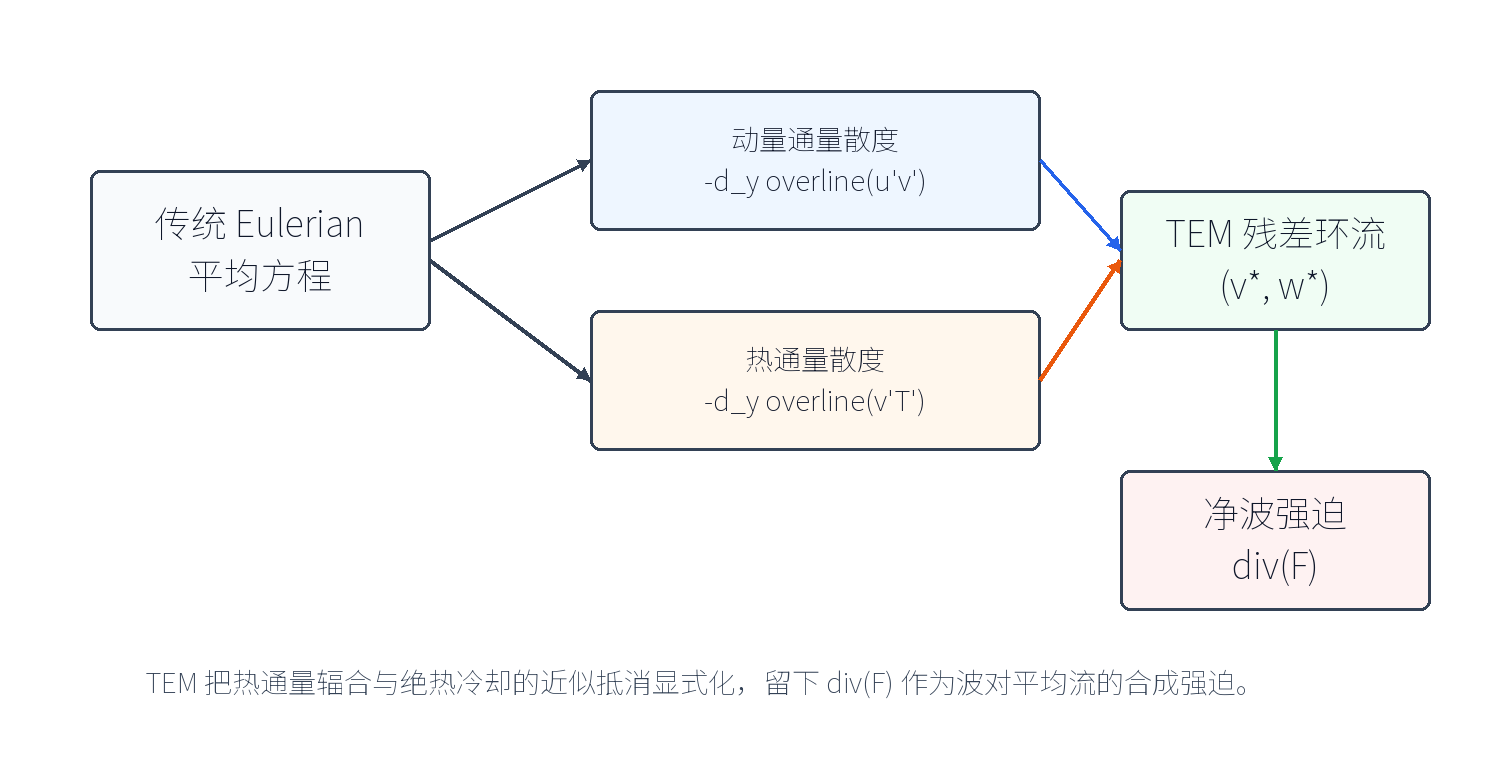
\includegraphics[width=0.92\linewidth]{fig1_tem_vs_eulerian.png}
  \caption{传统 Eulerian 平均与 TEM 的诊断差异。TEM 将热通量辐合与绝热冷却的近似抵消显式化，留下 $\nabla\cdot\bF$ 作为波对平均流的合成强迫。}
\end{figure}

\section{基本假设}

\subsection{Holton/TEM 准地转形式}

\begin{enumerate}
  \item 使用中纬度 $\beta$ 平面近似，基本运动满足准地转尺度关系。
  \item 采用纬向平均，任意变量分解为
  \begin{equation}
    A=\mean{A}+A',
  \end{equation}
  其中上划线表示纬向平均，撇号表示扰动量。
  \item 平均态近似满足地转平衡和静力平衡，因此满足热成风约束：
  \begin{equation}
    f_0\frac{\p\mean{u}}{\p z}
    +\frac{R}{H}\frac{\p\mean{T}}{\p y}=0.
  \end{equation}
  \item Holton 的常用写法采用 log-pressure 垂直坐标，背景密度为 $\rho_0(z)$，标高为 $H$。
  \item 在传统 Eulerian 平均的准地转尺度下，年龄地转平均经圈环流的平流项、显式垂直涡旋通量散度等高阶项可先忽略；未解析的小尺度涡动阻力 $\mean{X}$ 可保留。
  \item 静力稳定度由浮力频率 $N$ 描述。
\end{enumerate}

\subsection{垂直通量推广形式}

刘式适教材第 8.9 节进一步把 E-P 通量视为综合表征 Rossby 波动量和热量在经向、垂直方向输送的矢量场。该推广仍以波-基本气流相互作用为背景，并保留纬向平均与扰动分解：
\begin{equation}
  u=\mean{u}+u',\quad
  v=\mean{v}+v',\quad
  w=\mean{w}+w',\quad
  \theta=\mean{\theta}+\theta'.
\end{equation}

先讨论准地转条件下由经向动量输送和经向热量输送构成的 E-P 通量，再推广到显式保留垂直动量通量 $\mean{u'w'}$ 和垂直热通量 $\mean{\theta'w'}$ 的一般情形。

\section{物理量设定}

\begin{table}[H]
  \centering
  \caption{主要物理量和符号}
  \begin{tabular}{ll}
    \toprule
    符号 & 含义 \\
    \midrule
    $x$ & 纬向坐标 \\
    $y$ & 经向坐标，北向为正 \\
    $z$ & 垂直坐标；Holton 中常用 log-pressure 坐标 \\
    $\mean{u}$ & 平均纬向风 \\
    $\mean{v},\mean{w}$ & Eulerian 平均经向、垂直速度 \\
    $u',v',w'$ & 扰动速度 \\
    $T'$ 或 $\theta'$ & 扰动温度或扰动位温 \\
    $q',\mean{q}$ & 扰动准地转位涡、平均准地转位涡 \\
    $\psi'$ & 扰动流函数 \\
    $\rho_0$ & 背景密度 \\
    $N^2$ & 静力稳定度 \\
    $f_0$ & 参考科氏参数 \\
    $\mean{X}$ & 摩擦或未解析涡动造成的平均纬向力 \\
    $v^*,w^*$ & TEM 残差经圈环流 \\
    $\bF$ & Holton/TEM 形式的 E-P flux \\
    $\bJ_1$ & 经向动量和经向热量输送构成的 E-P 型通量 \\
    $\bJ_2$ & 显式垂直动量和垂直热量输送构成的 E-P 型通量 \\
    \bottomrule
  \end{tabular}
\end{table}

\section{从 Eulerian 平均到 TEM}

\subsection{传统 Eulerian 平均方程}

准地转、纬向平均后的纬向动量方程可写为
\begin{equation}
  \frac{\p\mean{u}}{\p t}
  -f_0\mean{v}
  =-\frac{\p\mean{u'v'}}{\p y}
  +\mean{X}.
\end{equation}

热力方程可写为
\begin{equation}
  \frac{\p\mean{T}}{\p t}
  +N^2\frac{H}{R}\mean{w}
  =-\frac{\p\mean{v'T'}}{\p y}
  +\frac{\mean{J}}{c_p}.
\end{equation}

这两个方程会把同一个波-平均流相互作用拆成两个看似独立的过程：动量通量改变平均风，热通量改变平均温度。但热成风约束要求平均风和平均温度协同变化，所以需要一个能直接诊断净强迫的形式。

\subsection{TEM 残差环流}

TEM 的关键步骤是把涡旋热通量的一部分吸收到残差经圈环流中：
\begin{align}
  v^*
  &=\mean{v}
  -\rho_0^{-1}\frac{R}{H}
  \frac{\p}{\p z}
  \left(
    \frac{\rho_0\mean{v'T'}}{N^2}
  \right),\\
  w^*
  &=\mean{w}
  +\frac{R}{H}
  \frac{\p}{\p y}
  \left(
    \frac{\mean{v'T'}}{N^2}
  \right).
\end{align}

残差环流不是普通 Eulerian 平均速度，而是更接近真实物质输送的平均环流。它显式表达了涡旋热通量辐合与平均垂直运动绝热冷暖之间的近似抵消关系。残差环流满足
\begin{equation}
  \frac{\p v^*}{\p y}
  +\rho_0^{-1}\frac{\p(\rho_0 w^*)}{\p z}=0.
\end{equation}

代入残差环流定义后，TEM 动量方程成为
\begin{equation}
  \frac{\p\mean{u}}{\p t}
  -f_0v^*
  =\rho_0^{-1}\nabla\cdot\bF+\mean{X}.
\end{equation}

热力方程成为
\begin{equation}
  \frac{\p\mean{T}}{\p t}
  +N^2\frac{H}{R}w^*
  =\frac{\mean{J}}{c_p}.
\end{equation}

于是涡旋动量通量和涡旋热通量不再分别解释平均流变化，而是通过同一个组合 $\nabla\cdot\bF$ 进入平均纬向动量方程。

\section{E-P flux 的定义与物理意义}

Holton 的 TEM 形式中，E-P flux 是经圈平面 $(y,z)$ 内的二维矢量：
\begin{equation}
  \bF=F_y\bj+F_z\bk,
\end{equation}
其中
\begin{align}
  F_y&=-\rho_0\mean{u'v'},\\
  F_z&=\rho_0 f_0\frac{R}{H}\frac{\mean{v'T'}}{N^2}.
\end{align}

其中 $F_y$ 与经向涡旋动量通量相反号，$F_z$ 与涡旋热通量成正比。需要特别区分：TEM 中的 $F_z$ 不是简单的垂直动量通量 $\mean{u'w'}$，而是热通量经由热成风和平衡关系转化出的垂直波活动传播分量。

\begin{figure}[H]
  \centering
  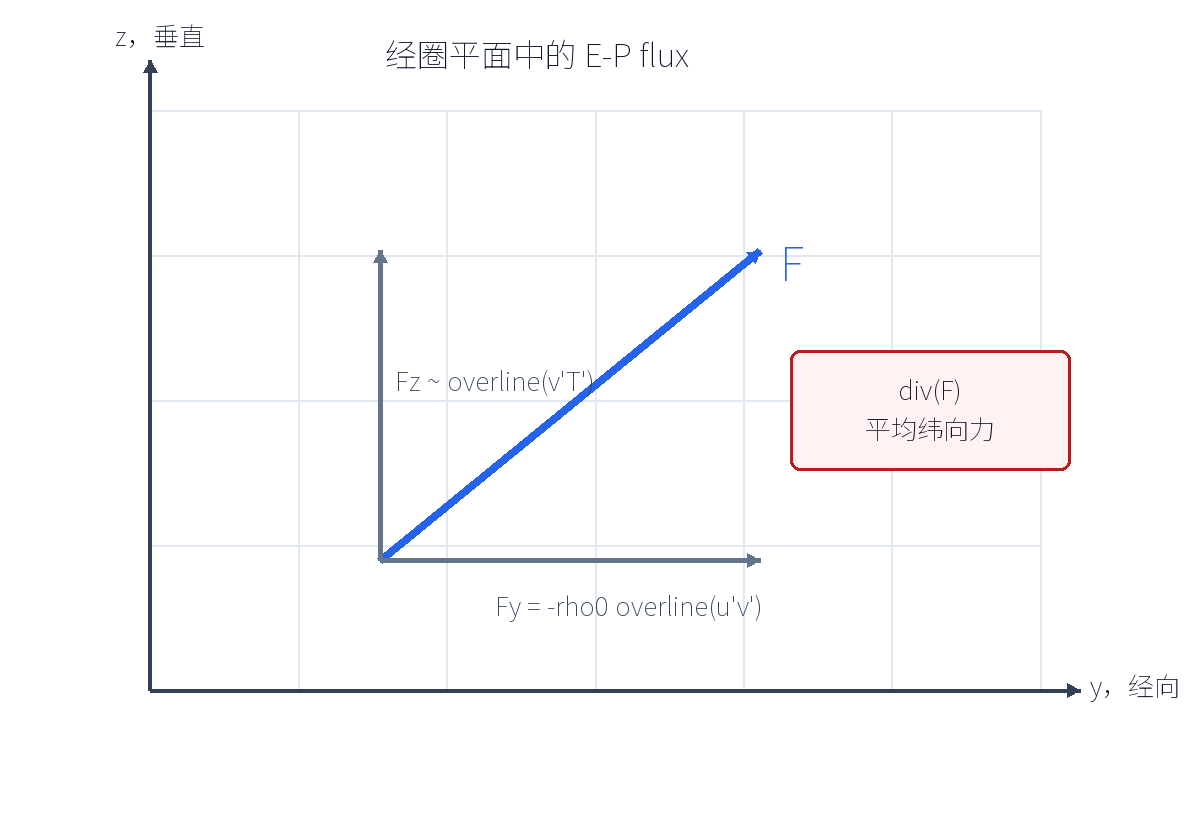
\includegraphics[width=0.84\linewidth]{fig2_ep_flux_vector.png}
  \caption{经圈平面中的 E-P flux。$F_y$ 由经向动量通量给出，$F_z$ 由经向热通量给出，$\nabla\cdot\bF$ 对应波对平均纬向流的净强迫。}
\end{figure}

准地转位涡扰动通量与 E-P flux 散度满足
\begin{equation}
  \mean{v'q'}=\rho_0^{-1}\nabla\cdot\bF.
\end{equation}

这说明大尺度波动对平均纬向流的强迫，等价于涡旋准地转位涡的经向输送。若没有涡旋位涡通量，绝热准地转条件下平均位涡分布不能被波动改变；若存在非零位涡通量，平均流必然调整。

\section{显式垂直通量运输的推广}

刘式适教材中首先定义经向输送矢量
\begin{equation}
  \bJ_1
  =-\mean{u'v'}\,\bj
  +\frac{f_0}{\p\theta_0/\p z}\mean{\theta'v'}\,\bk.
\end{equation}

它与 Holton 的准地转 TEM 形式对应，但使用位温 $\theta$ 和 $\p\theta_0/\p z$ 表达稳定度约束。

进一步考虑显式垂直通量运输时，引入
\begin{equation}
  \bJ_2
  =-\mean{u'w'}\,\bj
  +\frac{f_0}{\p\theta_0/\p z}\mean{\theta'w'}\,\bk.
\end{equation}

这里的 $\bJ_2$ 才是由垂直动量通量和垂直热通量构成的额外输送项。它说明平均位涡或平均基本流不仅受经向输送影响，也受垂直输送的空间不均匀性影响。

\begin{figure}[H]
  \centering
  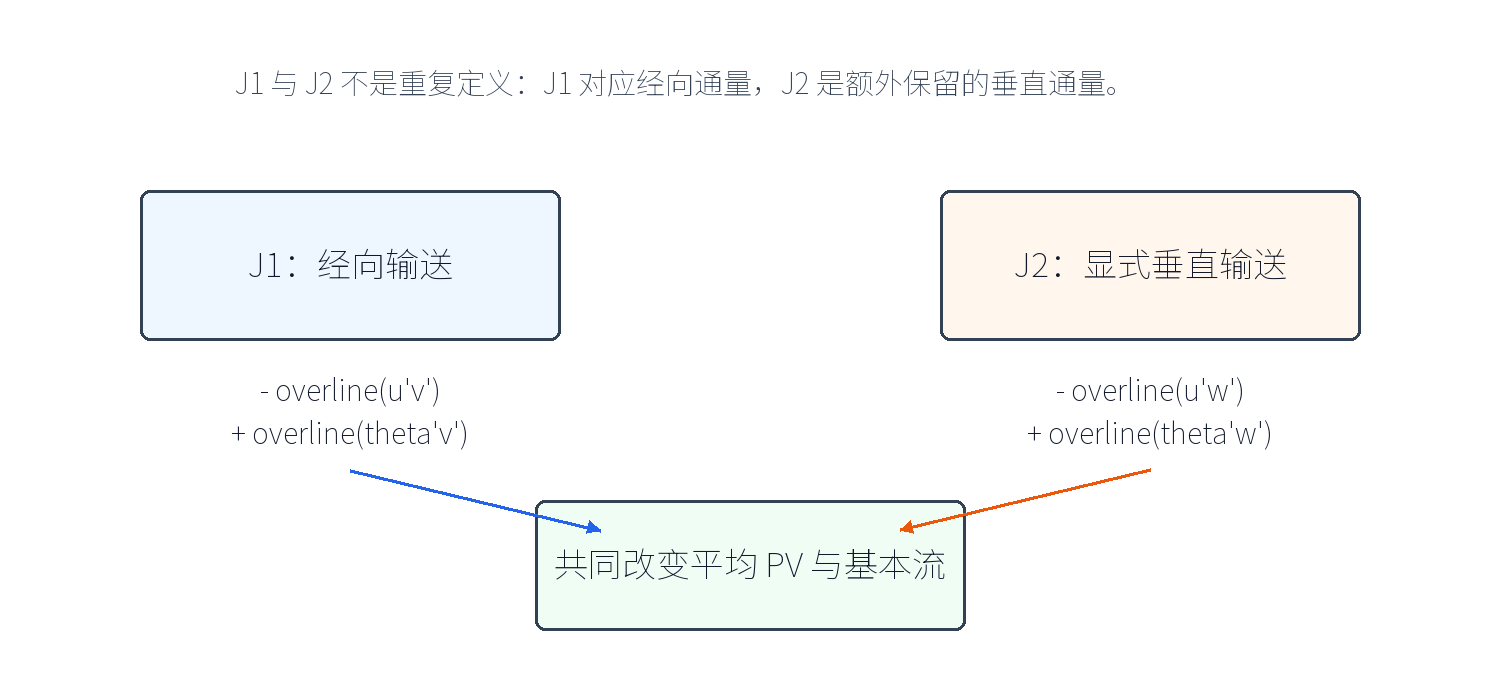
\includegraphics[width=0.92\linewidth]{fig3_j1_j2_comparison.png}
  \caption{$\bJ_1$ 与 $\bJ_2$ 的物理含义。$\bJ_1$ 对应经向动量/热量输送，$\bJ_2$ 对应显式垂直动量/热量输送。}
\end{figure}

在线性化准地转位涡守恒中，
\begin{equation}
  \left(
    \frac{\p}{\p t}
    +\mean{u}\frac{\p}{\p x}
  \right)q'
  +v'\frac{\p\mean{q}}{\p y}=0.
\end{equation}

乘以 $q'$ 并纬向平均，可得到扰动位涡拟能 $E_p$ 的变化：
\begin{align}
  \frac{\p E_p}{\p t}+\mean{q'v'}&=0,\\
  \mean{q'v'}&=\nabla\cdot\bJ_1,\\
  \frac{\p E_p}{\p t}+\nabla\cdot\bJ_1&=0.
\end{align}

因此，$\nabla\cdot\bJ_1<0$ 表示 E-P 通量辐合，扰动位涡拟能增加；$\nabla\cdot\bJ_1>0$ 表示 E-P 通量辐散，扰动位涡拟能减小。

在更一般的情形中，平均准地转位涡随时间的变化不仅依赖 $\nabla\cdot\bJ_1$ 的经向变化，还依赖 $\nabla\cdot\bJ_2$ 的垂直变化：
\begin{equation}
  \frac{\p\mean{q}}{\p t}
  =
  -\frac{\p}{\p y}
  \left(\nabla\cdot\bJ_1\right)
  -\frac{\p}{\p z}
  \left(\nabla\cdot\bJ_2\right).
\end{equation}

其中
\begin{equation}
  \nabla\cdot\bJ_2
  =
  -\frac{\p\mean{u'w'}}{\p y}
  +\frac{f_0}{\p\theta_0/\p z}
  \frac{\p\mean{\theta'w'}}{\p z}.
\end{equation}

这条式子是加入垂直通量运输后的关键结论：动量和热量输送及其空间分布不均匀，可以通过经向和垂直两个方向共同改变平均准地转位涡，从而改变基本气流。

\begin{figure}[H]
  \centering
  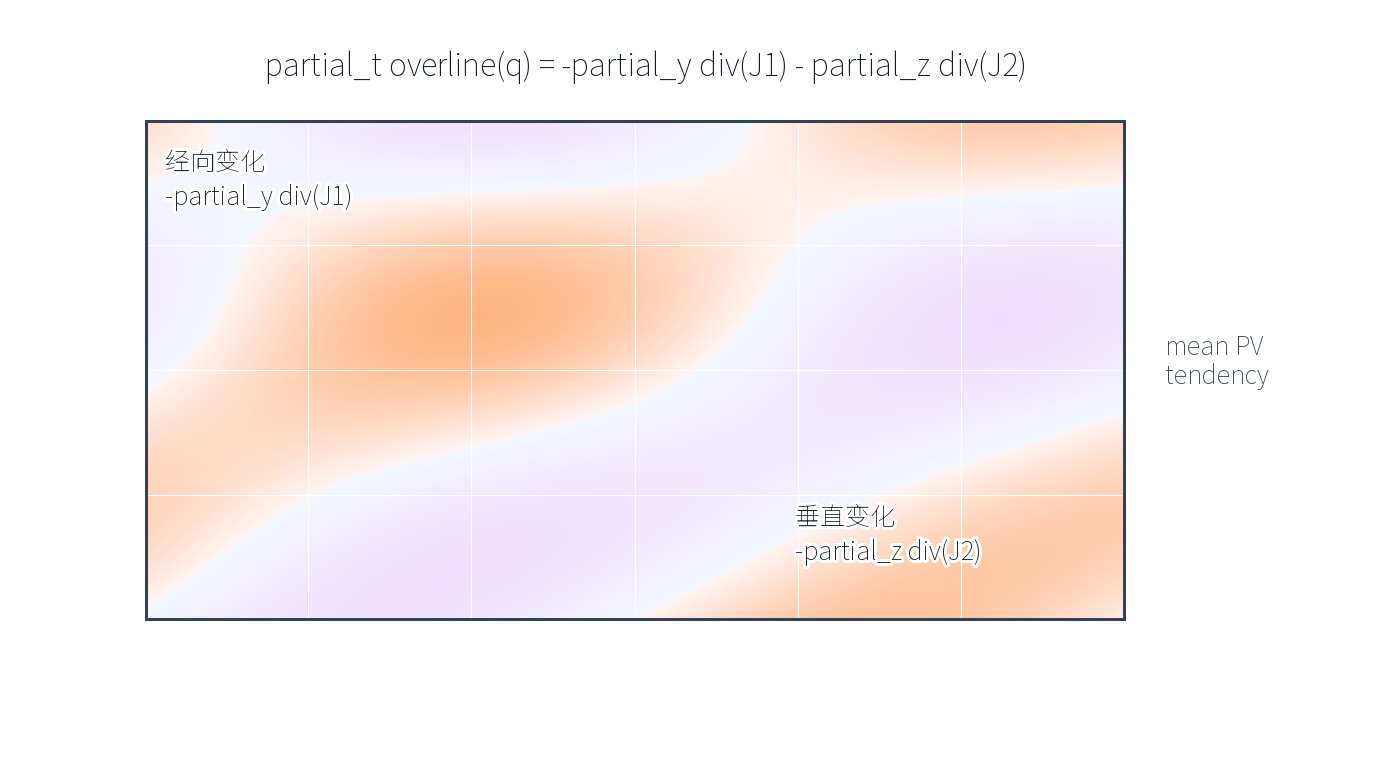
\includegraphics[width=0.86\linewidth]{fig4_qbar_feedback.png}
  \caption{$\nabla\cdot\bJ_1$ 的经向变化与 $\nabla\cdot\bJ_2$ 的垂直变化共同控制平均位涡倾向。}
\end{figure}

\section{重要结论}

\begin{enumerate}
  \item E-P flux 的方向近似表示波活动传播方向。在经圈平面中，E-P flux 的方向可用于判断 Rossby 波活动或波能量传播方向。
  \item E-P flux 散度是波对平均流的纬向力。$\nabla\cdot\bF>0$ 表示东向加速，$\nabla\cdot\bF<0$ 表示西向减速或阻力。
  \item E-P flux 将热通量和动量通量的补偿关系显式化。分析波-平均流相互作用时，关键不是单独看 $\mean{u'v'}$ 或 $\mean{v'T'}$，而是看 $\nabla\cdot\bF$ 或 $\mean{v'q'}$。
  \item E-P flux 与残差环流共同维持平均经圈环流。在季节平均尺度上，E-P flux 散度产生的纬向力常近似由残差经圈环流的科氏力平衡。
  \item 显式垂直通量运输会改变平均位涡和基本气流。加入 $\bJ_2$ 后，即使经向通量作用不强，垂直动量通量或垂直热通量的高度不均匀也能改变平均 PV，并通过热成风平衡反馈到平均风和温度结构。
\end{enumerate}

\section{与 coherent tilt 诊断的关系}

涡旋本体应由扰动位涡 $q'$、扰动流函数 $\psi'$ 或扰动地转速度 $\bV'_g$ 定义，而不是由背景平均位涡 $\mean{q}$ 定义。背景 $\mean{q}$ 的角色是控制扰动 PV 的传播、折射、相位调整和反馈平均流。

准地转涡旋本体可写为
\begin{equation}
  q'
  =
  \nabla_h^2\psi'
  +
  \frac{\p}{\p z}
  \left(
    \frac{f_0^2}{N^2}
    \frac{\p\psi'}{\p z}
  \right).
\end{equation}

扰动地转速度由扰动流函数给出：
\begin{equation}
  u'_g=-\frac{\p\psi'}{\p y},
  \qquad
  v'_g=\frac{\p\psi'}{\p x}.
\end{equation}

设第 $z$ 层涡旋核心位置为
\begin{equation}
  \br_c(z,t)=\left(x_c(z,t),y_c(z,t)\right).
\end{equation}

若各层核心近似落在一条三维直线上，则其水平投影可写成
\begin{equation}
  \br_c(z,t)\approx\br_0(t)+z\bm{b}(t),
  \qquad
  \ep(t)=\frac{\bm{b}(t)}{|\bm{b}(t)|}.
\end{equation}

令涡旋核心水平速度为 $\bV_c=\p\br_c/\p t$，则
\begin{equation}
  \frac{\p\bm{b}}{\p t}
  =
  \frac{\p\bV_c}{\p z},
  \qquad
  \ep(t)
  \parallel
  \int_0^t
  \frac{\p\bV_c}{\p z}(t')\,\dd t'.
\end{equation}

也就是说，projection direction vector 的方向由涡旋核心速度的垂直切变累积决定。

\begin{figure}[H]
  \centering
  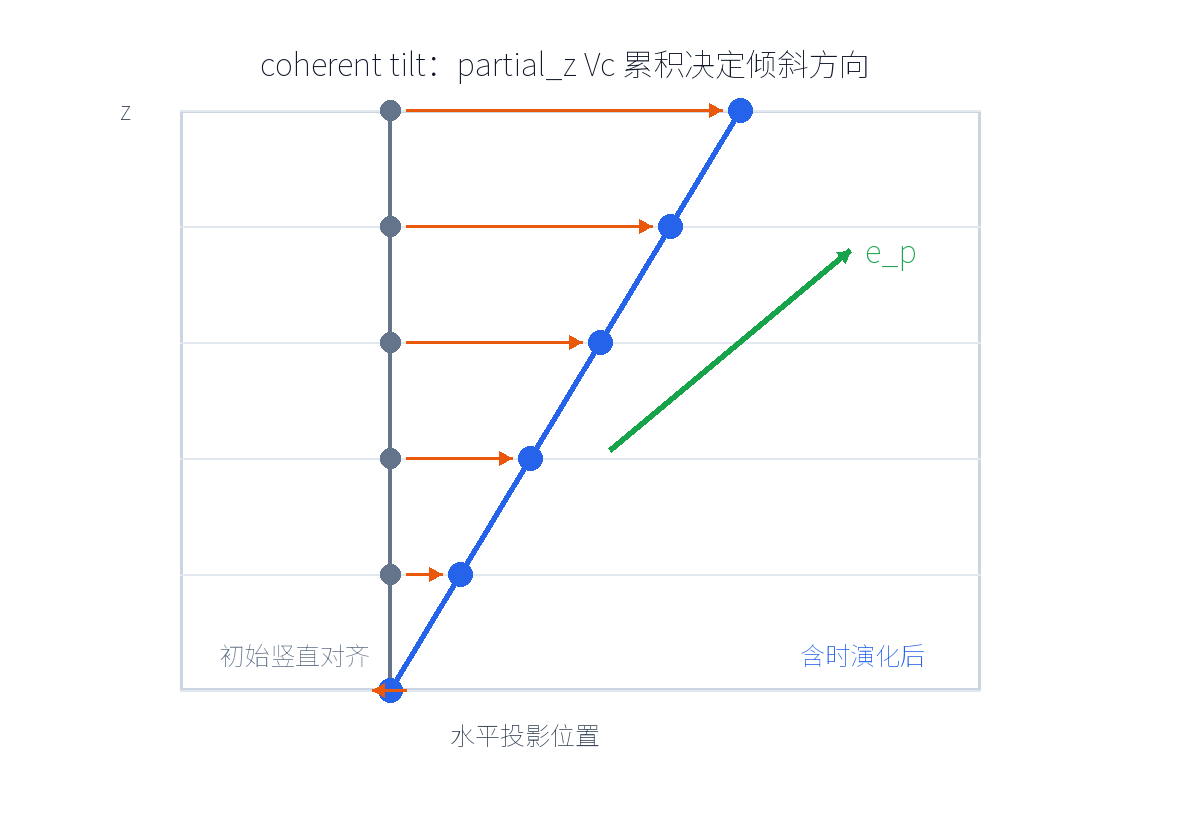
\includegraphics[width=0.78\linewidth]{fig5_coherent_tilt.png}
  \caption{coherent tilt 诊断示意。初始竖直对齐的涡旋核心，在 $\p_z\bV_c$ 的累积作用下形成倾斜但仍 coherent 的结构。}
\end{figure}

更完整地，涡旋核心速度可分解为
\begin{equation}
  \bV_c
  \approx
  \mean{\bV_g}
  +\bV_{\mathrm{intrinsic}}[q']
  +\bV_a
  +\bV_{\mathrm{eddy\ drift}}.
\end{equation}

因此 coherent 直线倾斜的强条件是
\begin{equation}
  \frac{\p^2\bV_c}{\p z^2}\approx 0.
\end{equation}

若基本流平流主导，则可近似退化为
\begin{equation}
  \frac{\p\mean{u}}{\p z}\ne 0,
  \qquad
  \frac{\p^2\mean{u}}{\p z^2}\approx 0.
\end{equation}

E-P flux 在这里不是直接定义涡旋中心，而是通过 $\nabla\cdot\bF$、$\nabla\cdot\bJ_1$ 和 $\nabla\cdot\bJ_2$ 改变平均流和平均 PV，再反馈到 $\p_z\bV_c$。因此 coherent tilt 要求这些反馈在高度上足够平滑；若某层出现强 E-P flux 辐合/辐散或强垂直通量散度突变，涡旋轴更容易弯曲或失去 coherent。

\section{一句话总结}

E-P flux 理论的精髓是：Rossby 波不是分别通过动量输送和热量输送独立改变平均流，而是通过一个合成通量的散度改变平均纬向力和平均位涡；在准地转 TEM 中这个合成通量已有由热通量表示的垂直分量 $F_z$，而在进一步考虑显式垂直通量运输时，还要加入由 $\mean{u'w'}$ 与 $\mean{\theta'w'}$ 构成的 $\bJ_2$，使平均位涡变化同时受经向和垂直通量散度的空间变化控制。

\end{document}
